\documentclass{article}
\usepackage[final]{neurips}
\usepackage[framemethod=tikz]{mdframed}
\usepackage{lipsum}
\definecolor{mycolor}{rgb}{0.122, 0.435, 0.698}
\newmdenv[innerlinewidth=0.5pt, roundcorner=4pt,linecolor=mycolor,innerleftmargin=6pt,
innerrightmargin=6pt,innertopmargin=6pt,innerbottommargin=6pt]{mybox}
\usepackage[utf8]{inputenc} % allow utf-8 input
\usepackage[T1]{fontenc}    % use 8-bit T1 fonts
\usepackage[hidelinks]{hyperref}       % hyperlinks
\usepackage{url}            % simple URL typesetting
\usepackage{booktabs}       % professional-quality tables
\usepackage{amsfonts}       % blackboard math symbols
\usepackage{nicefrac,tcolorbox}       % compact symbols for 1/2, etc.
\usepackage{amsmath}
\usepackage{enumitem}
\usepackage{microtype}      % microtypography
\usepackage{graphicx,caption,fontspec}
\usepackage{xepersian}
\settextfont{XB Niloofar}
\setdigitfont{XB Niloofar}
\raggedbottom
\newenvironment{parind}{%
	\par%A
	\leftskip=0mm\rightskip=7mm
	\noindent\ignorespaces}{%
	\par}

\title{
	\vspace{-0.8em}
	تمرین امتیازی 2 - درس نظریه گروه‌ها - دکتر رضاخانی
	\\
	{\normalsize
		\textbf{مهلت تحویل:
			تا دوشنبه ۲۱ خرداد سال ۱۴۰۳ - ساعت ۵۹:۲۳
			\\
			\vspace{-0.4em}
			از طریق سامانه
			\href{https://cw.sharif.edu/}{درس‌افزار شریف}
		}
	}
	\vspace{-0.6em}
}


\newtcolorbox{boxes}[3][]
{
	colframe = #2!25,
	colback  = #2!10,
	coltitle = #2!40!black,  
	title    = {\textbf{#3}},
	#1,
}

\newenvironment{exercise}[3][\unskip]{%
	\par
	\noindent
	\textbf{تمرین
		#1
		[- امتیاز] 
		\def\temp{#3}\ifx\temp\empty
		: 
		\else
		: #3 \vspace{0.5em} \\ \noindent
		\fi
}}{}

\author{
	حسین محمدی\\
	\lr{
		\href{mailto:hossein.mohammadi.00427@gmail.com}{\texttt{	hossein.mohammadi.00427@gmail.com}}} \\
	\And
	زهرا کبیری\\
	\lr{
		\href{mailto:kabiri.zahra98@gmail.com}{ \texttt{kabiri.zahra98@gmail.com}}}\\
}

\begin{document}
	
	
	\begin{minipage}{0.1\textwidth}% adapt widths of minipages to your needs
		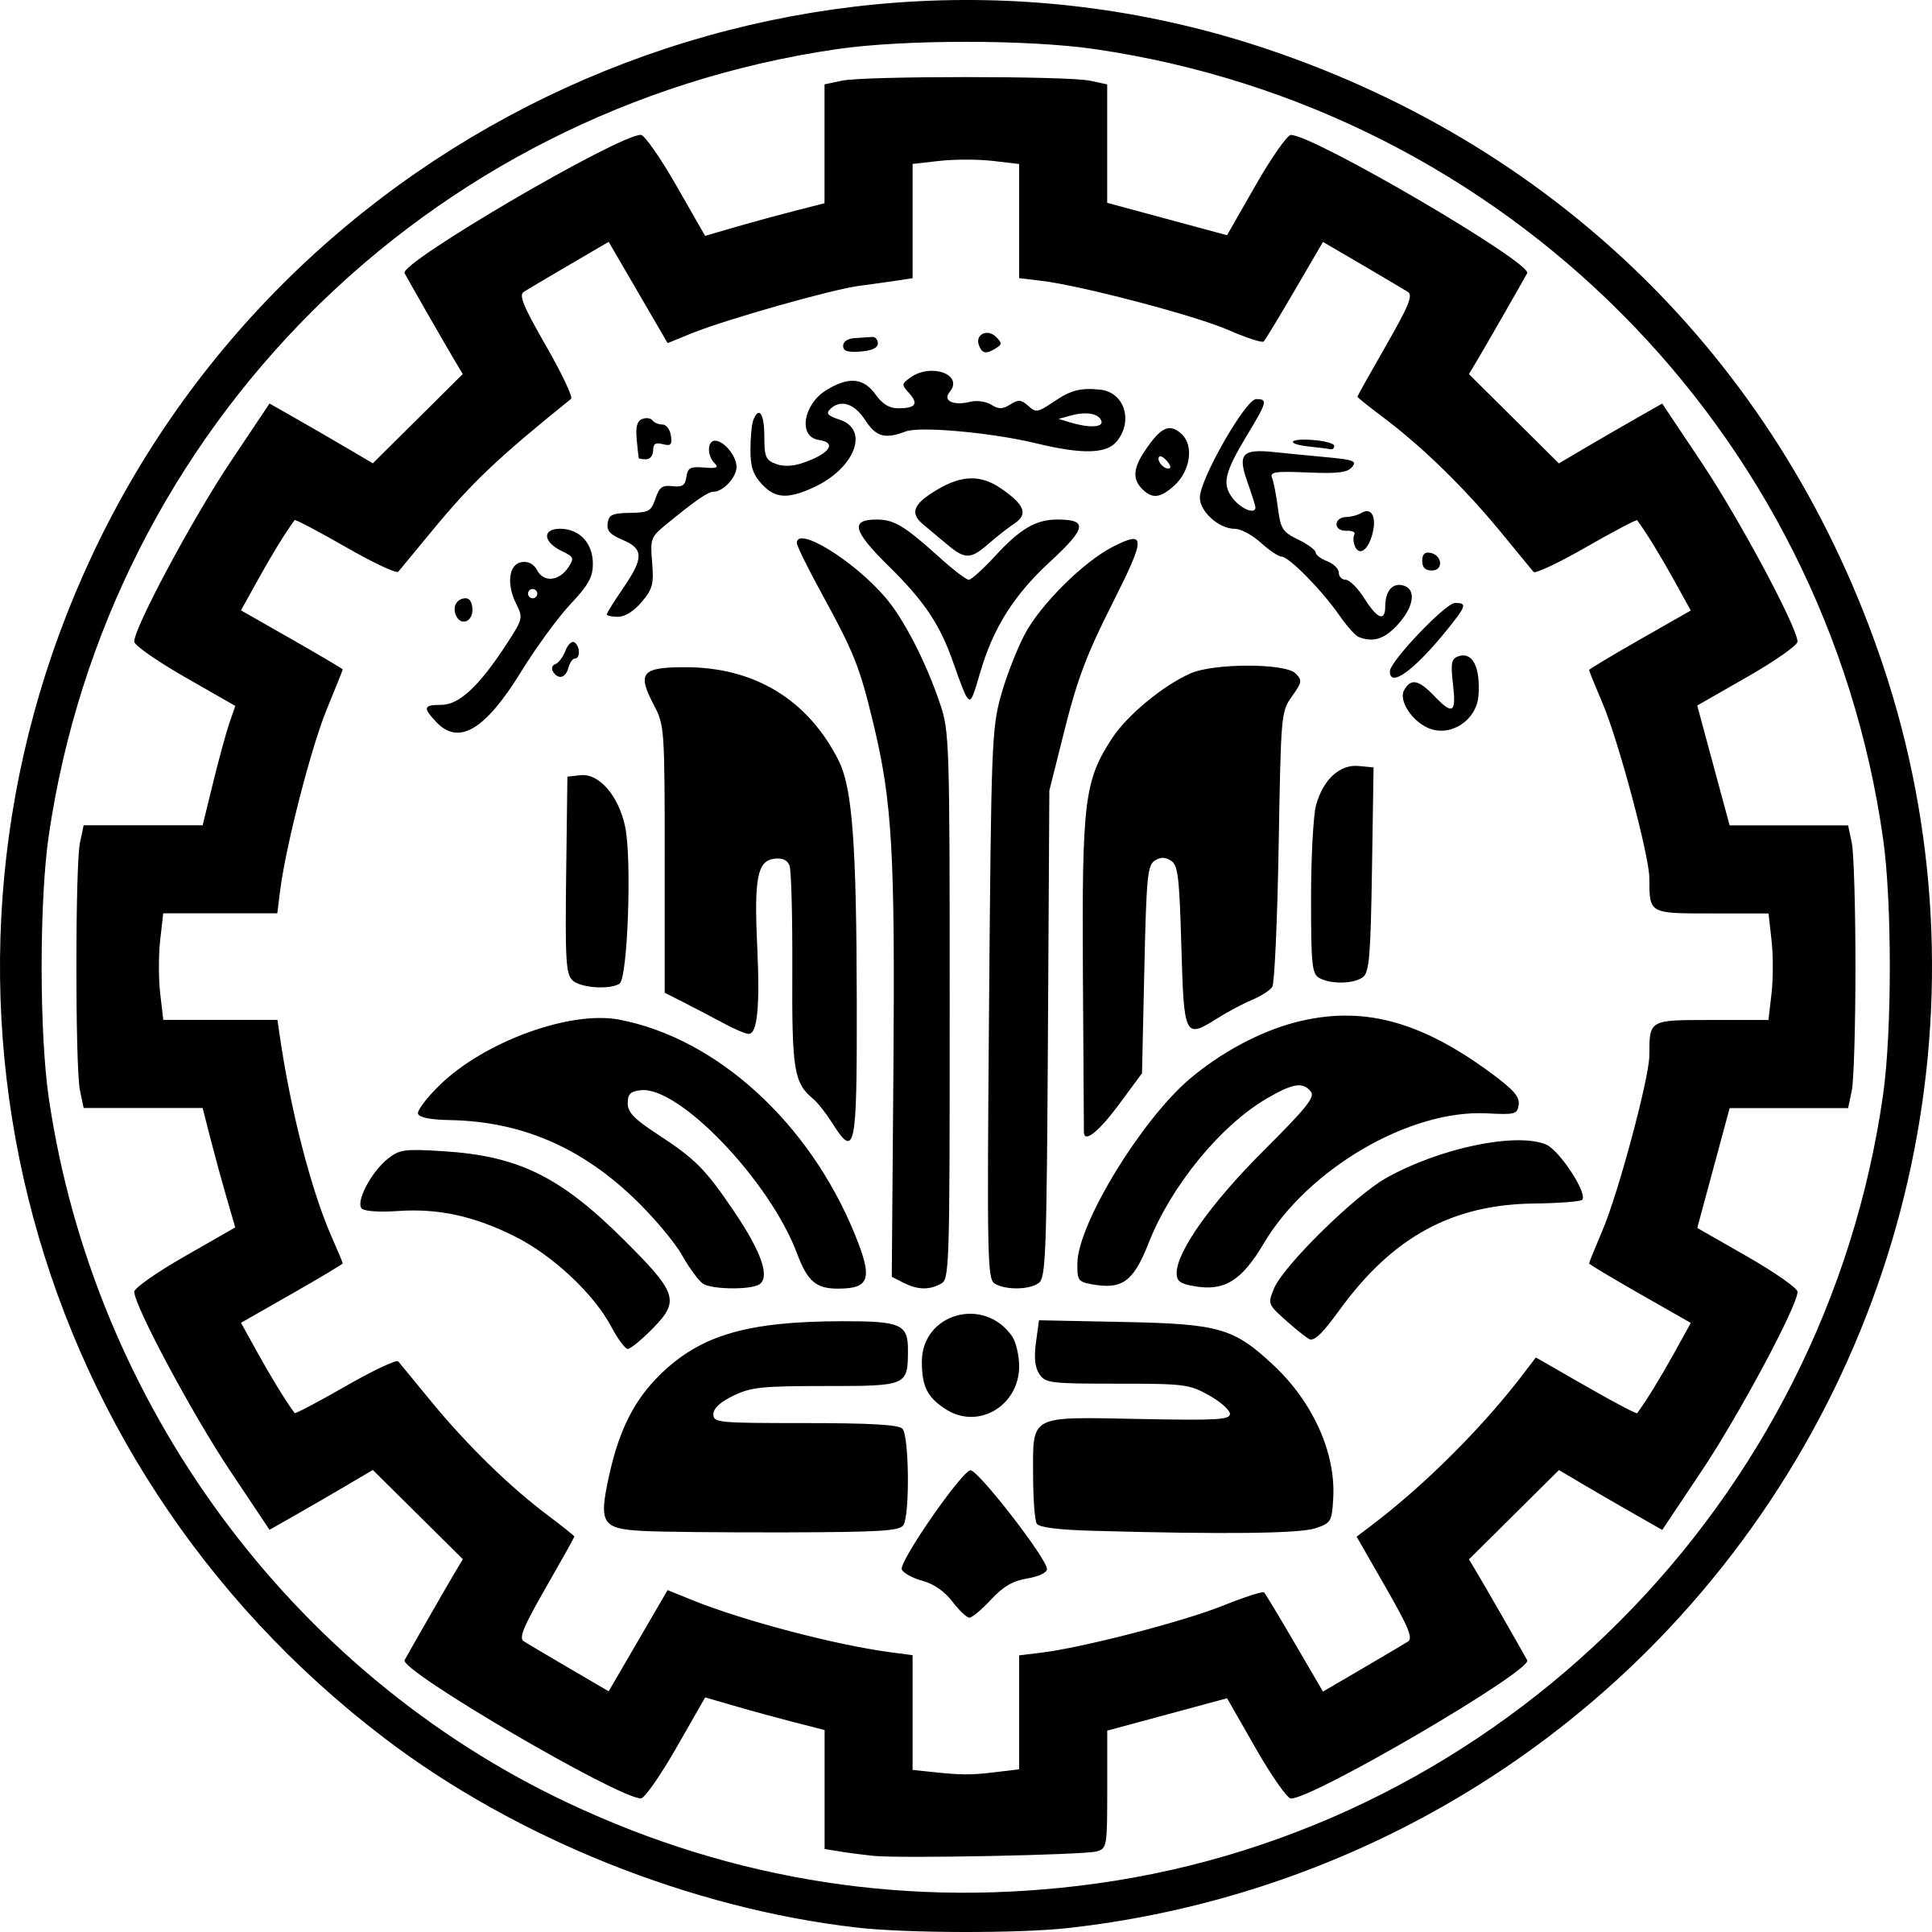
\includegraphics[width=1.1cm]{sharif-logo.png}
	\end{minipage}%
	\hfill%
	\begin{minipage}{0.9\textwidth}\raggedleft
		دانشگاه صنعتی شریف\\
		زمستان ۱۴۰۲ - بهار ۱۴۰۳\\
	\end{minipage}
	
	\makepertitle
	
	\noindent
	برای جبران نمرات از دست رفته، به حل سوالات امتیازی بپردازید. با این شرایط که:
	\begin{enumerate}
		\item برای کسب نمره‌ی کامل از سوالات زیر \underline{9 سوال}  انتخاب و حل کنید. 
		\item در مورد سوالات چندبخشی، حل باید به ترتیب انجام بگیرد و نمی‌توان بدون حل یک قسمت، از نتیجه‌اش در قسمت‌های بعدی استفاده کرد. 
		
	\end{enumerate}
	
	
	\begin{exercise}[$14''$]{20}{لمِ
			\lr{Burnside}
		}
		در این سوال، قصد داریم یک نتیجه‌ی مهم از اثر گروه روی مجموعه‌ها  را بررسی کنیم.
		\begin{mdframed}
			گروه متناهی $G$ رو مجموعه‌ی 
			$S$
			اثر می‌کند. مجموعه‌ی اعضایی از $S$ که تحت اثر یک عضوِخاص از گروه $G$ ثابت می‌مانند، با 
			$\text{\lr{fix}}(g)$
			نشان می‌دهیم.
			\[
			\text{\lr{fix}}(g) = \{s\in S \; \big| \; g.s=s\}
			\]
			هم‌چنین، 
			$S/G$
			، نمایانگر مجموعه‌ی تمامی مدارهای این اثر است.
		\end{mdframed}
		لمِ 
		\lr{Burnside}
		را ثابت کنید.
		\begin{parind}
			برای گروه متناهی $G$ که روی مجموعه‌ی متناهی $S$ اثر می‌کند:
			\[
			|S/G| = \frac{1}{|G|} \sum_{g\in G}|\text{\lr{fix}}(g)|
			\]
		\end{parind}
		
		\noindent
		(\textbf{راهنمایی:}
		با 
		$\sum_{g\in G} \text{\lr{fix}}(g)$
		شروع کنید و سعی کنید آن را برحسب جمع روی پایدارسازهای عناصر 
		$S$ بازنویسی کنید. در نهایت از قضیه مدار-پایدارساز استفاده کنید.
		)
		
	\end{exercise}
	
	\begin{exercise}[$15''$]{20}{مسائل رنگی از اثر گروه روی مجموعه (۱)}
		تعداد رنگ‌آمیزیِ متمایز شکلِ
		\eqref{fig1}
		را 
		( که کاشی‌کاری مثلث متساوی الاضلاع است) به‌دست بیاورید؛ یعنی به چند روشِ متمایز می‌توان هفت مثلث متساوی‌الاضلاع را رنگ کرد. توجه کنید که منظور از رنگ‌آمیزی‌ِ متمایز، رنگ‌آمیزی‌هایی است که با دوران و بازتاب این شکل، به همدیگر تبدیل نشوند. بدیهی هست که باید فرض کنید تعداد
		$n$ رنگ متمایز دارید، و بایستی با کمک لم
		\lr{Burnside}
		، رنگ آمیزیها را بشمارید.
		
		\noindent
		(\textbf{راهنمایی:}
		حل مسئله را با اعمال کردن لم 
		\lr{Burnside}
		به گروه $D_3$ که گروه تقارنی این شکل است، شروع کنید.
		)
		
		\begin{figure}[h]
			\centering
			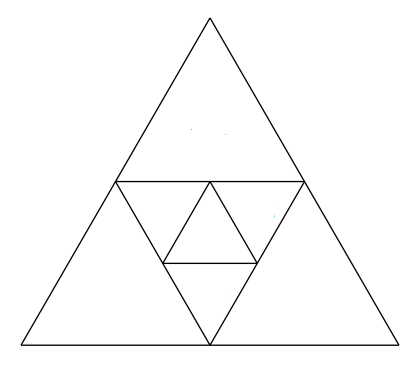
\includegraphics[width=15em]{Pics/1.png}
			\caption{مثلث متساوی‌الاضلاع کاشی شده برای مسئله‌ی رنگ‌آمیزی}
			\label{fig1}
		\end{figure}
		
	\end{exercise}
	\begin{exercise}[$16''$]{20}{مسائل رنگی از اثر گروه روی مجموعه (۲)}
		به‌عنوان کاربردی دیگر، مسئله‌ی «رنگ‌آمیزی گردن‌بند» را حل می‌کنیم. نخی به شکل حلقه داریم که به تعداد دلخواه مهره در آن هست، در این مسئله می‌خواهیم ببینیم که با رنگ‌های مجزا، به چند روش می‌توان این گردن‌بند را رنگ‌آمیزی کرد. مثل بالا، تحت دوران و چرخش گردن‌بند، رنگ‌آمیزی‌های متمایز، با هم معادل نیستند. (مثلا در رنگ‌آمیزی‌های شکل 
		\ref{pic2}
		، 
		به دو گردن‌بند معادل می‌رسیم؛ چون با دوران (یا بازتاب) این دو گردن‌بند به همدیگر تبدیل می‌شوند.
		)
		
		\begin{figure}[h]
			\centering
			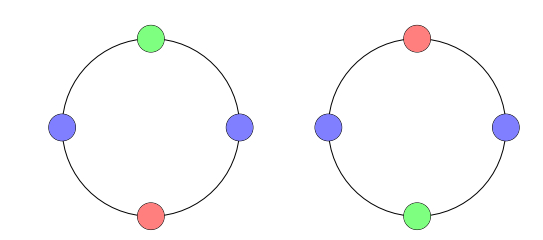
\includegraphics[width=32em]{Pics/2.png}
			\caption{رنگ‌آمیزیِ معادل دو گردن‌بند با چهار مهره و سه رنگ.}
			\label{pic2}
		\end{figure}
		
		حالا تعداد رنگ‌آمیزی‌های متمایز یک گردن‌بند ۶ مهره‌ای، با $n$ رنگ را بدست بیاورید. این رابطه را به $m$ مهره هم تعمیم دهید.
	\end{exercise}
	\begin{exercise}[$17''$]{20}{پیوستگی با دو معنای متفاوت}
		\noindent
		در درس با مفهوم فضای توپولوژیک و همچنین ظرایف آن آشنا شدید؛ حالا می‌خواهیم یک تمرین نسبتا معروف و ساده را با هم بررسی کنیم.
		
		نشان دهید که تعریف آنالیزی پیوستگی با تعریف توپولوژیکی آن معادل است.
		\begin{mdframed}
			\textbf{تعریف توپولوژیک پیوستگی:}
			می‌گوییم تابع
			$f: X \mapsto Y$ 
			یک تابع پیوسته است، اگر برای هر مجموعه‌ی باز از فضای مقصد،
			$U \subset Y$
			،
			پیش‌تصویر
			\LTRfootnote{Preimage}
			آن در مبدا باز باشد.
			\footnote{از  آقای آرشا نیک‌سا بابت توجه‌شان و نشان دادن اشتباه تایپی این بخش متشکریم.}
			یعنی 
			$V \equiv f^{-1}(U) = \{
			x\in X \; | \; f(x) \in U
			\}$
			با توپولوژی فضای مبدا یک فضای باز محسوب شود.
			
			\textbf{تعریف آنالیزی پیوستگی:}
			تابع
			$f: X \mapsto Y$
			پیوسته است اگر برای هر نقطه‌ی 
			$p \in X$
			گزاره‌ی زیر برقرار باشد.
			\[
			\forall \epsilon>0, \forall x \in X, \exists \delta>0 : d_X(x,p)<\delta \xrightarrow{\quad} d_Y(f(x),f(p))<\epsilon
			\]
			که در آن 
			$d_X$
			و
			$d_Y$
			به‌ترتیب متریک‌های روی فضای مبدا و مقصد هستند.
			
		\end{mdframed}
		
	\end{exercise}
	
	
	\begin{exercise}[$18''$]{20}{یک‌ریختی جبر‌هایِ لی}
		\vspace{-1em}
		\begin{parind}
			الف)	نشان دهید جبر لی گروه‌های 
			$\mathfrak{sl}(2,\mathbb{C})$ 
			و 
			$\mathfrak{so}(3,\mathbb{C})$ 
			یک‌ریخت هستند. 
			
			
			ب)	نشان دهید 
			$SU(1,1,\mathbb{C}) $ 
			با 
			$SL(2,\mathbb{R}) $ 
			یک‌ریخت است.
		\end{parind}
		
		
	\end{exercise}
	
	\begin{exercise}[$19''$]{20}{}
		گروه 
		$S^1= \{(x_1,x_2) \; | \; x_1^2+x_2^2=1\}$ 
		را در نظر بگیرید
		\footnote{می‌دانیم هر نقطه روی دایره‌ی واحد را با عددی مختلط که فازِخالص است می‌توان نشان داد؛ عمل ضرب گروهی، همان ضرب اعداد مختلط است.}
		. فضایی را که از دیفیومورفیسم‌هایی
		\LTRfootnote{\lr{Diffeomorphism}  $: S^1 \to S^1$} 
		تشکیل شده که جهت زاویه‌ای را حفظ می‌کند 
		$\text{Diff}^+ (S^1)$ 
		می‌نامیم. 
		ضرب این 
		گروه از ترکیب این دیفیومورفیسم‌ها به دست ‌می‌آید. در نهایت یک گروه لی بینهایت بعدی خواهیم داشت. جبر لی مربوط به آن فضای میدان‌های برداری روی 
		$S^1$ 
		است. یک زیرجبر
		\LTRfootnote{Subalgebra} 
		لی از ترکیب جبر لی 
		$\text{Diff}^+ (S^1)$ 
		چنین است:
		\begin{equation*}
			L = \left\{ f(z) \frac{d}{dz} \; : \; f(z) \in \mathbb{C}[z,z^{-1}] \right\}
		\end{equation*}
		این یک زیرفضا از فضای میدان‌های برداری روی 
		$S^1$ 
		است با توجه به اینکه 
		$S^1$ 
		دایره واحد در 
		$\mathbb{C}$ 
		است.  پایه 
		$\{L_n\}_{n \in \mathbb{Z}}$ 
		برای این جبر را اینطور انتخاب می‌کنیم: 
		\begin{equation*}
			L_n := - z^{n+1}\frac{d}{dz}
		\end{equation*} 
		جابه‌جاگر 
		$[L_n,L_m]$ 
		را بیابید.
	\end{exercise}
	
	
	\begin{exercise}[$20''$]{20}{}
		الف)
		عضوی از گروه لی 
		$GL(2,\mathbb{R})$ 
		را در نظر بگیرید: 
		\begin{equation*}
			A=\left(
			\begin{matrix}a&b\\c&d\\\end{matrix}
			\right) \in GL(2,\mathbb{R})
		\end{equation*}
		در نتیجه 
		$\det A \neq 0$. 
		تبدیل موبیوس
		\LTRfootnote{Möbius} 
		اینطور عمل می‌کند:
		\begin{equation*}
			z \to \frac{az+b}{cz+d}
		\end{equation*}
		\begin{parind}
			الف)نشان دهید اگر تبدیل موبیوس را روی صفحه مختلط توسعه داده شده
			\footnote{در حقیقت این فضا همان کره ریمان است؛ که شامل تمامی اعداد مختلط است که با فشرده‌سازی تک‌نقطه‌ای، بی‌نهایت هم جزئی از فضاست.} 
			$\mathbb{C}\cup \{ \infty \}$ 
			اثر دهیم یک گروه تحت ترکیب توابع خواهد ساخت. 
			\\
			ب) نشان دهید این گروه با گروه خارج قسمت 
			$GL(2,\mathbb{R}) / Z_{GL(2,\mathbb{R})}$ 
			یکریخت است. 
			$Z$
			مرکز گروه 
			$GL(2,\mathbb{R})$ 
			است.
		\end{parind}
		
		
	\end{exercise}
	
	
	\begin{exercise}[$21''$]{20}{}
		جبر لی 
		$\mathfrak{su}(5)$ 
		از تمام ماتریس‌های 
		$5 \times 5$ای 
		تشکیل شده که: 
		\begin{equation*}
			X^{\dag}=-X \quad \quad trX =0
		\end{equation*}
		یک پایه متعامد برای 
		$\mathfrak{su}(5)$
		معرفی کنید. 
		ضرب داخلی فضای ماتریسی را چنین در نظر بگیرید:
		‌
		\[\left<X_j,X_k \right>=\text{Tr}(X_jX_k^{\dag})
		\]
	\end{exercise}
	
	\begin{exercise}[$22''$]{20}{گروه‌های تقارنی در نظریه‌ی میدان}
		با کاربرد‌های گروه‌ها در نظریه‌های فیزیکی آشناتر شویم و ساده‌ترین مدلی را که تقارن
		$\text{U}(1)$
		دارد، بررسی می‌کنیم.لاگرانژی این کنش را در زیر می‌بینیم.
		
		\[
		\mathcal{L}_{\phi} = (\partial_\mu {\phi})^* (\partial^\mu {\phi}) - \frac12 M^2 \phi^*\phi,
		\]
		
	\end{exercise}
	\noindent
	\begin{parind}
		الف) اول نشان دهید که این لاگرانژی تحت تبدیل 
		$e^{i\varphi} \in \text{U}(1)$
		به شکل زیر، ناورداست.
		\begin{equation*}
			\begin{aligned}
				{\phi} &\xrightarrow{\quad } e^{i\varphi}{\phi} \\
			\end{aligned}
		\end{equation*}
		
		ب) جریان و بار نوتر مربوط به این تقارن پیوسته‌ی سرتاسری را پیدا کنید.
		
		ج) نشان‌دهید که تحت تبدیل موضعی،
		$\phi \xrightarrow{\quad } e^{i\varphi(x)}{\phi}$
		،
		کنش ناوردا نمی‌ماند.
		
		د) حالا تقارن سرتاسری را پیمانه‌ای می‌کنیم. یعنی کنش را طوری اصلاح می‌کنیم که تحت تبدیلِ تقارنی با پارامتر‌های وابسته به فضازمان، همچنان ناوردا باشد.  برای ارتقای تقارن‌ها به تقارن موضعی، مشتق‌های عادی را به مشتق هموردا تبدیل می‌کنیم:
		\[
		\partial_\mu {\phi} \xrightarrow{\quad } D_\mu {\phi} = (\partial_\mu  +\frac{i}{e}  A_\mu)  {\phi}
		\]
		که در این روابط، $e$ ثابتی است که قوت برهمکنش را مشخص می‌کند. همچنین میدان‌های جدید $A_\mu$
		را معرفی کرده‌ایم؛ بنابراین لازم است جمله‌ی جنبشی مربوط به آن را هم در لاگرانژی وارد کنیم. این‌جمله‌ی جنبشی به شکل زیر است
		\footnote{منظور از توان دو رساندن این است که اندیس‌های پایین
			$\mu,\nu$
			با اندیس‌های بالای 
			$\mu,\nu$
			\lr{contract}
			شوند.
		}.
		\[
		\mathcal{L}_{\text{\small gauge}} = -\frac14 \big(
		\partial_\mu A_\nu - \partial_\nu A_\mu
		\big)^2
		\]
		
		بنابراین لاگرانژی جدید که تحت تقارن موضعی 
		$\text{SU}(2)$
		ناورداست، به شکل زیر است:
		\[
		\mathcal{L}_{\text{Tot}} =  \mathcal{L}_{\text{\small gauge}} + \mathcal{L}_{\phi}[\partial \xrightarrow{\quad} D]
		\]
		که منظور از جمله‌ی آخری، تبدیل مشتق‌های عادی به همورداست.
		
		تا اینجا همه‌اش مقدمات بود، حالا سوال اصلی این است: نشان دهید که لاگرانژی 
		$\mathcal{L}_{\text{Tot}} $
		تحت تبدیلات بی‌نهایت کوچکِ زیر ناورداست.
		\begin{equation*}
			\begin{aligned}
				\phi &\xrightarrow{\quad} {\phi} + i \varphi (x) {\phi} \\ 
				A_\mu (x) &\xrightarrow{\quad} A_\mu(x) + ie \partial_\mu \varphi(x).
			\end{aligned}
		\end{equation*}
		که در آن، پارامتر تبدیلِ بی‌نهایت کوچک
		،$\varphi(x)$،
		وابسته به فضازمان هستند.
	\end{parind}

	
	
	\begin{exercise}[$23''$]{20}{}
		\newcommand{\cev}[1]{\reflectbox{\ensuremath{\vec{\reflectbox{\ensuremath{#1}}}}}}
		براکت مویال 
		\LTRfootnote{Moyal Bracket}
		(که به آن براکت سینوس هم گفته می‌شود)
		 اینطور تعریف می‌شود
		\footnote{از آقایان شهمیری و اشتری برای تذکرشان ممنونیم.}
		: 
		
		\begin{equation*}
			[f(\mathbf{p},\mathbf{q}),g(\mathbf{p},\mathbf{q})]_{\text{M}}:=
			 \frac{2}{\hbar}f(\mathbf{p},\mathbf{q})
			\sin \left( \frac{\hbar}{2}\;(
			\cev{\partial}_{\mathbf{q}}.\vec{\partial}_{\mathbf{p}}
			-\cev{\partial}_{\mathbf{p}}.\vec{\partial}_{\mathbf{q}})
			\right)
			g(\mathbf{p},\mathbf{q})
		\end{equation*}
		که در آن 
		\begin{equation*}
			\partial_{\mathbf{q}}.\partial_{\mathbf{p}} :=
			\sum^n_{j=1} \frac{\partial}{\partial q_j}\frac{\partial}{\partial p_j}, 
			\quad \quad
			\partial_{\mathbf{p}}.\partial_{\mathbf{q}} :=
			\sum^n_{j=1} \frac{\partial}{\partial p_j}\frac{\partial}{\partial q_j}
		\end{equation*}
		همانطور که می‌بینید در حد 
		$\hbar \to 0$ 
		براکت مویال همان براکت پواسون می‌شود. چند ویژگی براکت مویال این است که:
		\begin{enumerate}
			\item
			نسبت به ورودی‌های 
			$f$ 
			و 
			$g$ 
			پادمتقارن است. 
			\item 
			در اتحاد جاکوبی صدق می‌کند.
		\end{enumerate}
		براکت مویال یک جبر لی بی‌نهایت بعدی را مشخص می‌کند. 
		\\
		همیلتونی زیر را در نظر بگیرید:
		\begin{equation*}
			H(\mathbf{p},\mathbf{q}) = \frac{1}{2}p_1^2+\frac{1}{2}p_2^2
			+\frac{16}{3}q_2^3+q_1 q_2^2 + \mu q_1^{-2}
		\end{equation*}
		تابع 
		$I(\mathbf{p},\mathbf{q})$ 
		را این بگیرید:
		\begin{equation*}
			I(\mathbf{p},\mathbf{q}) =p_1^4+
			4(q_1^2 q_2 + \mu q_1^{-2})p_1^2 
			-\frac{4}{3}q_1^3 p_1 p_2
			-\frac{4}{3}q_1^4 q_2^2 
			+\frac{8}{3}\mu q_2
			-\frac{2}{9}q_1^6
			+4 \mu^2 q_1^{-4}
		\end{equation*}
		براکت مویال 
		$[I,H]_{\text{M}}$ 
		را به دست آورید و نتیجه‌را در قیاس با براکت پواسون به بحث بگذارید.
	\end{exercise}
	
	\begin{exercise}[$24''$]{20}{تبدیلات هم‌تافته در حل مسائل مکانیک کلاسیک}
		در این سوال، تبدیلی کانونیک به ما در حل یک مسئله‌ی خاص از مکانیک کلاسیک کمک می‌کند.
		\begin{parind}
			الف)
			نشان‌دهید که تبدیلات زیر از مختصه‌های مکان و تکانه
			$(q^1,q^2,p_1,p_2)$
			به 
			$(Q^1,Q^2,P_1,P_2)$
			، یک تبدیل هم‌تافته است.
			\begin{equation*}
				\begin{aligned}
					Q^1 &= q^1\cos\alpha - \frac{p_2}{\beta}\sin\alpha, \quad P_1 = \beta q^2 \sin\alpha + p_1\cos\alpha
					\\
					Q^2 &= q^2\cos\alpha - \frac{p_1}{\beta}\sin\alpha, \quad P_2 = \beta q^1 \sin\alpha + p_2\cos\alpha
				\end{aligned}
			\end{equation*}
			ب) ذره‌ای به جرمِ $m$ و بارِ $e$
			تحت اثر پتانسیل نوسانگر هماهنگ 
			$\frac12 m\omega_0^2 \big[
			(q^1)^2+ (q^2)^2
			\big]$
			و میدان مغناطیسی با پتانسیلِ برداری 
			$\mathbf{A} = (0,hq^1,0)$
			($h$ ثابت است.)
			حرکت می‌کند.
			از تبدیلات کانونیک بالا استفاده کنید و با تعریف 
			$\tan 2\alpha = \frac{2m\omega}{eh}$ و انتخابِ مناسبِ $\beta$
			، مسیر حرکت این ذره را پیدا کنید برای دو حد 
			$h=0$ و $h \to \infty$
			این مسیر را توصیف کنید
			\footnote{از آقای طالبی برای یادآوری اشتباه تایپی ممنونیم.}
			.
		\end{parind}
	\end{exercise}
	
	
	\begin{exercise}[$25''$]{20}{}
	در فیزیک نسبیت خاص،‌ کنش یک ذره متحرک را با طول ویژه جهان‌خط آن نشان می‌دهیم. از انگیزه‌های این کار این بوده که فضا‌زمان روشی برای نگاه کردن به مکان و زمان از یک عینک است،‌ به طوری که نمی‌توان مکان و زمان را مستقل و جداگانه از هم بررسی کرد. در نتیجه انتظار داریم کنش یک اسکالر لورنتزی باشد که در نهایت ما را به عبارت زیر می‌رساند:
	\begin{equation*}
	    S \propto \int_{b}^{a}ds = \int_{b}^{a}\sqrt{c^2 dt^2-dx^2}
	\end{equation*}
	اما مشکلی وجود دارد که بعد کنش و طول ویژه متفاوت است. یک ثابت 
	$mc$ 
	برای یکی شدن دو طرف تساوی در انتگرال ضرب می‌کنیم.
		\begin{equation*}
	    S = -mc\int_{b}^{a}\sqrt{c^2 dt^2-dx^2}
	\end{equation*}
	علامت منفی برای همخوانی کنش با حد کلاسیک 
	$\frac{v}{c}\ll1$ 
	است.
	\begin{parind}
	
	الف)‌ فرم این عبارت را به حالت آشنای 
	$S = \int_{b}L dt$ 
	در بیاورید و لاگرانژی نسبیتی به دست آمده را بنویسید. \\
	ب) نشان دهید این لاگرانژی تحت انتقال در مکان 
	$x \to x+\delta x$ 
	متقارن است.  بار نوتر مربوط به این تقارن را به دست آورید. \\
	ج) نشان دهید این لاگرانژی تحت انتقال در زمان 
	$t \to t+\delta t$ 
	متقارن است. بار نوتر مربوط به آن را به دست آورید. ارتباط کمیت‌هایی که در بخش ب و ج به دست آوردید را با چهاربردار تکانه نسبیتی توضیح دهید. \\
	د) آیا در حد 
	$\frac{v}{c}\ll1$ 
	عبارت‌هایی که به دست آوردید به مقدار کلاسیکی نظیرشان می‌رسند؟ 
	\footnote{
	دیدن عبارت 
	$E=mc^2$ معروف خالی از لطف نیست! 
		یعنی حتی در حد کلاسیک هم می‌توان گفت جرم باید شکلی از انرژی باشد و در نتیجه می‌تواند به شکل‌های دیگر انرژی از جمله انرژی جنبشی تبدیل شود. یکی از نتایج این نوع نگاه کردن به جرم در گرانش خودش را نشان می‌دهد. در گرانش نیوتونی تنها اجسام جرم‌دار گرانش را حس می‌کنند. اما از آن‌جا که در نسبیت خاص جرم هم شکلی از انرژی است، احتمالا این تصور دور از انتظار نیست که شکل‌های دیگر انرژی نیز بتوانند از گرانش اثر بگیرند یا روی آن اثر بگذارند. به عنوان مثال فوتون‌های بدون جرم (اما پرانرژی) تحت تاثیر گرانش قرار می‌گیرند و گرانش نیوتونی هیچ توضیحی برای آن نمی‌تواند ارائه کند. تئوری کامل‌تری که می‌تواند این ارتباط را توضیح دهد نسبیت عام است.
	}
\end{parind}
	\end{exercise}
	
	
	\begin{exercise}[$26''$]{20}{}
		مولدهای گروه همدیس 
		\LTRfootnote{conformal group} 
		(که خود جبرِلی هستند)
		در فضازمان
		$d$-بعدی 
		از این قرارند:
		\begin{equation*}
			\begin{matrix}\left(\text{\lr{Translation}}\right)&P_\mu=-i\ \partial_\mu\\
				\left(\text{\lr{Dilation}}\right)&D=-i\ x^\mu\partial_\mu\\
				\left(\text{\lr{Rotation}}\right)&L_{\mu\nu}=i(x_\mu\partial_\nu-x_\nu\partial_\mu)\\
				\left(\text{\lr{Special Conformal Transformation}}\right) & K_\mu=-i({2x}_\mu x^\nu\partial_\nu-x^2\partial_\mu)\\\end{matrix}
		\end{equation*}
		\noindent
		\begin{parind}
		الف)‌ نشان دهید رابطه‌های جابه‌جاگری زیر برای این مولدها برقرار است: 
		\begin{equation*}
			\begin{aligned}
				[D,P_{\mu}]&=i P_{\mu}\\
				[D,K_{\mu}]&=-i K_{\mu}\\
				[K_{\mu},P_{\nu}]&=2i(\eta _{\mu \nu} D - L_{\mu \nu})\\
				[K_{\rho},L_{\mu \nu}]&=i(\eta _{\rho \mu} K_{\nu} - \eta _{\rho \nu} K_{\mu})\\
				[P_{\rho},L_{\mu \nu}]&=i(\eta _{\rho \mu} P_{\nu} - \eta _{\rho \nu} P_{\mu})\\
				[L_{\mu \nu},L_{\rho \sigma}]&=i(\eta _{\nu \rho} L_{\mu \sigma} + \eta _{\mu \sigma} L_{\nu \rho} - \eta _{\mu \rho} L_{\nu \sigma} - \eta _{\nu \sigma} L_{\mu \rho})\\
			\end{aligned}
		\end{equation*}
		که در آن 
		$\eta _{\mu \nu}$ 
		متریک فضازمان است. \\
		ب) نشان دهید جبر گروه همدیس با 
		$SO(d+1,1)$ 
		یکریخت است.
		\\
		\indent
		راهنمایی: مولدهای گروه همدیس را چنین بنویسید 
		\begin{equation*}
			\begin{matrix}
				J_{\mu \nu}=L_{\mu \nu} &\quad J_{-1,\mu}=\frac{1}{2}(P_{\mu}-K_{\mu})\\
				J_{-1,0}=D &\quad J_{0,\mu}=\frac{1}{2}(P_{\mu}+K_{\mu})\\
			\end{matrix}
		\end{equation*}
		\indent
		که در آن 
		$J_{ab}=-J_{ba}$ 
		و 
		$a,b \in \{-1,0,1,...,d\}$. 
				\end{parind}
	\end{exercise}
	
	
	\begin{exercise}[$27''$]{20}{}
		نشان دهید هر یکی از موارد زیر گروه لی هستند: 
		\begin{enumerate}
			\item[1]
			هر فضای برداری متناهی بعد که ساختار گروه جمع‌پذیر
			\LTRfootnote{Additive group} 
			دارد، به خصوص 
			$\mathbb{R}^n$. 
			\item[2]
			مجموعه اعداد مختلط غیر صفر 
			$\mathbb{C}^*$ 
			با ضرب اعداد مختلط.
			\item[3]
			$G \times H$ 
			که در آن 
			$G$ 
			و 
			$H$ 
			گروه لی هستند و ضرب اعضای آن‌ها اینطور تعریف شده: 
			\begin{equation*}
				(g,h)(g',h')=(gg',hh')\quad: g,g' \in G, \quad h,h' \in H
			\end{equation*}
			تعمیم این حالت به تعداد دلخواه گروه‌های لی چنین است که اگر 
			$G_i$ 
			به ازای 
			$i\in \{1,...,n\}$ 
			گروه لی باشند آن‌گاه 
			$G_1 \times ... \times G_n$
			یک گروه لی است.
			\item[4]
			گروهِ 
			\lr{Toral} 
			یا
			$T^n = \underbrace{S^1 \times \dots \times S^1}_{ n \; \text{times}}$ 
			برای 
			$n \ge 1$. 
			\item[5]
			خودریختی‌های
			\LTRfootnote{Automorphism}
			 فضای برداری متناهی بعد روی 
			$\mathbb{R}$ 
			یا 
			$\mathbb{C}$ 
			$(\text{Aut}(V))$، 
			به خصوص 
			$\text{GL}(n,\mathbb{R})=\text{\lr{Aut}}_{\mathbb{R}}\mathbb{R}^n$ 
			و 
			$\text{GL}(n,\mathbb{C})=\text{\lr{Aut}}_{\mathbb{C}}\mathbb{C}^n$.
			\item[6]
			$K=\mathbb{R}^n \times GL(n,\mathbb{R})$ 
			برای 
			$n>1$ 
			که ساختار گروه این طور تعریف شده:
			\begin{equation*}
				(x,A)(x',A')=(x+Ax', AA')
			\end{equation*}
		\end{enumerate}
	\end{exercise}
	
	
	\begin{exercise}[$28''$]{20}{}
		$X$ 
		عضوی از جبر لی 
		$\mathfrak{sl}(2,\mathbb{R})$ 
		از گروه تبدیلات خطی حقیقی ویژه  
		$SL(2,\mathbb{R})$ 
		است. 
		$\exp(X)$ 
		را به دست آورید.
	\end{exercise}
	
	\begin{exercise}[$29''$]{20}{}
		$G$ 
		یک زیرگروه کاهش‌‌ناپذیر از 
		$GL(\mathcal{V},\mathbb{C})$ 
		است. اگر 
		$c \in GL(\mathcal{V})$ 
		مرکزساز 
		$G$ 
		باشد، نشان دهید وجود دارد
		$\gamma \in \mathbb{C} $ 
		که 
		$c=\gamma 1$. 
		به خصوص  بخش‌های کاهش‌ناپذیر یک گروه آبلی کاملا کاهش‌پذیر 
		$A \subseteq GL(\mathcal{V})$ 
		همگی از درجه‌ی ۱ هستند. در نتیجه 
		$A$ 
		مربوط به یک گروه قطری است اگر پایه 
		مناسبی برای 
		$\mathcal{V}$ 
		بگیریم. \\
		\indent
		راهنمایی: نشان دهید برای هر 
		$\alpha \in \mathbb{C}$ 
		قسمت 
		$\mathcal{V}(c- \alpha 1)$ 
		یک زیرفضای ناوردا برای 
		$G$ 
		است.
	\end{exercise}
	
	
	\begin{exercise}[$30''$]{}{}
		نشان‌دهید اگر $G$ یک زیرگروه ‌کاهش‌ناپذیر از گروهِ‌خطی روی فضایِ برداری 
		$\mathcal{V}$
		باشد؛ هر زیرگروه بهنجار از 
		$G$ یک زیرگروه کاملا کاهش‌پذیراست. همچنین نشان‌دهید که تعداد مولفه‌های کاهش‌پذیری این زیرگروهِ بهنجار، مرتبه‌ی گروه
		$G$
		را می‌شمارد.
		
	\end{exercise}
	
	\begin{boxes}{black}{آشنایی با برخی اصطلاحات در گروه‌های خطی}
		با برخی اصطلاحات در گروه‌های خطی آشنا می‌شویم؛ بعدها که با نمایش آشنا شدید، می‌بینید که نمایش چیزی جز یک همریختی بین گروه‌ها و گروهِ خطی نیست؛ بنابراین این اصطلاحات به طور طبیعی در آنجا هم استفاده خواهند شد.
		
		گروهِ خطی 
		$\text{GL}(n,\mathbb{R})$
		روی فضایِ برداری 
		$\mathcal{V}$
		که فضایی 
		$n$-بعدی 
		است اثر می‌کند؛ در اصطلاح می‌گوییم که اعضای گروه خطی (یا هر زیرگروهی از آن) از 
		\textbf
		{درجه‌ی
			\LTRfootnote{Degree}
			$\mathbf{n}$} هستند.
		
		حالا فرض ‌کنید گروه
		$G$، زیرگروهی از این گروهِ‌خطی باشد. در این‌صورت زیرفضایِ خطیِ 
		$\mathcal{W}
		$
		از فضای 
		$\mathcal{V}$ یک 
		\textbf{زیرفضای ناوردای گروه 
			$\mathbf{G}$
			\LTRfootnote{Invariant subspace of subgroup $G$}
		}
		نامیده می‌شود اگر\
		\LTRfootnote{$g\mathcal{W} = \{
			gw \; | \; w \in \mathcal{W}
			\}$} 
		$g\mathcal{W} = \mathcal{W}$
		برای هر 
		$g\in G$.
		در این حالت، تحدید‌کردن اثر اعضای گروهِ
		$G$ به 
		$\mathcal{W}$
		به ما زیرگروهی از 
		$\text{GL}(m,\mathcal{W})$
		می‌دهد؛ که در آن 
		$m = \dim(\mathcal{W})$.
		
		می‌گوییم زیرگروه $G$ یک \textbf{زیرگروه‌ِ کاهش‌ناپذیر
			\LTRfootnote{Irreducible subgroup}
		} است اگر به جز 
		$\mathcal{V}$
		و زیرفضایِ بدیهی
		،
		$\{\}$
		،
		زیرفضایِ ناوردای دیگری نداشته باشد.
		در غیرِاین‌صورت، به این زیرگروه، \textbf{زیرگروهِ کاهش‌پذیر
			\LTRfootnote{Reducible subgroup}
		} می‌گوییم.
		
		به‌ زیرگروهِ 
		$G$
		یک \textbf{زیرگروهِ کاملا‌کاهش‌پذیر
			\LTRfootnote{Compeletely reducible subgroup}
		}می‌گوییم اگر بتوان فضایِ برداری 
		$\mathcal{V}$
		را به‌شکل جمع مستقیم زیرفضاهایِ ناوردآی آن نوشت.
		\[
		\mathcal{V} = \oplus_{i=1}^k \mathcal{W}_i
		\]
		مشخصا، یک زیرگروهِ کاهش‌ناپذیر، کاملا کاهش‌پذیر هم هست. به تحدیدِ هر کدام از اعضای گروه $G$ به زیرفضاهای 
		$\mathcal{W}_i$،
		یک \textbf{مولفه‌های کاهش‌ناپذیرِ زیرگروه
			\LTRfootnote{Irreducible components of subgroup $G$}
		}
		$\mathbf{G}$
		می‌گوییم.
	\end{boxes}
	
	
	
	
	\vspace{1em}
\end{document}
